% Hardware
\chapter{Hardware}
\section{Existing Mount PCB}\label{sec:appendix_gs_pcb_existing}
\begin{figure}[!htb]
  \centering
  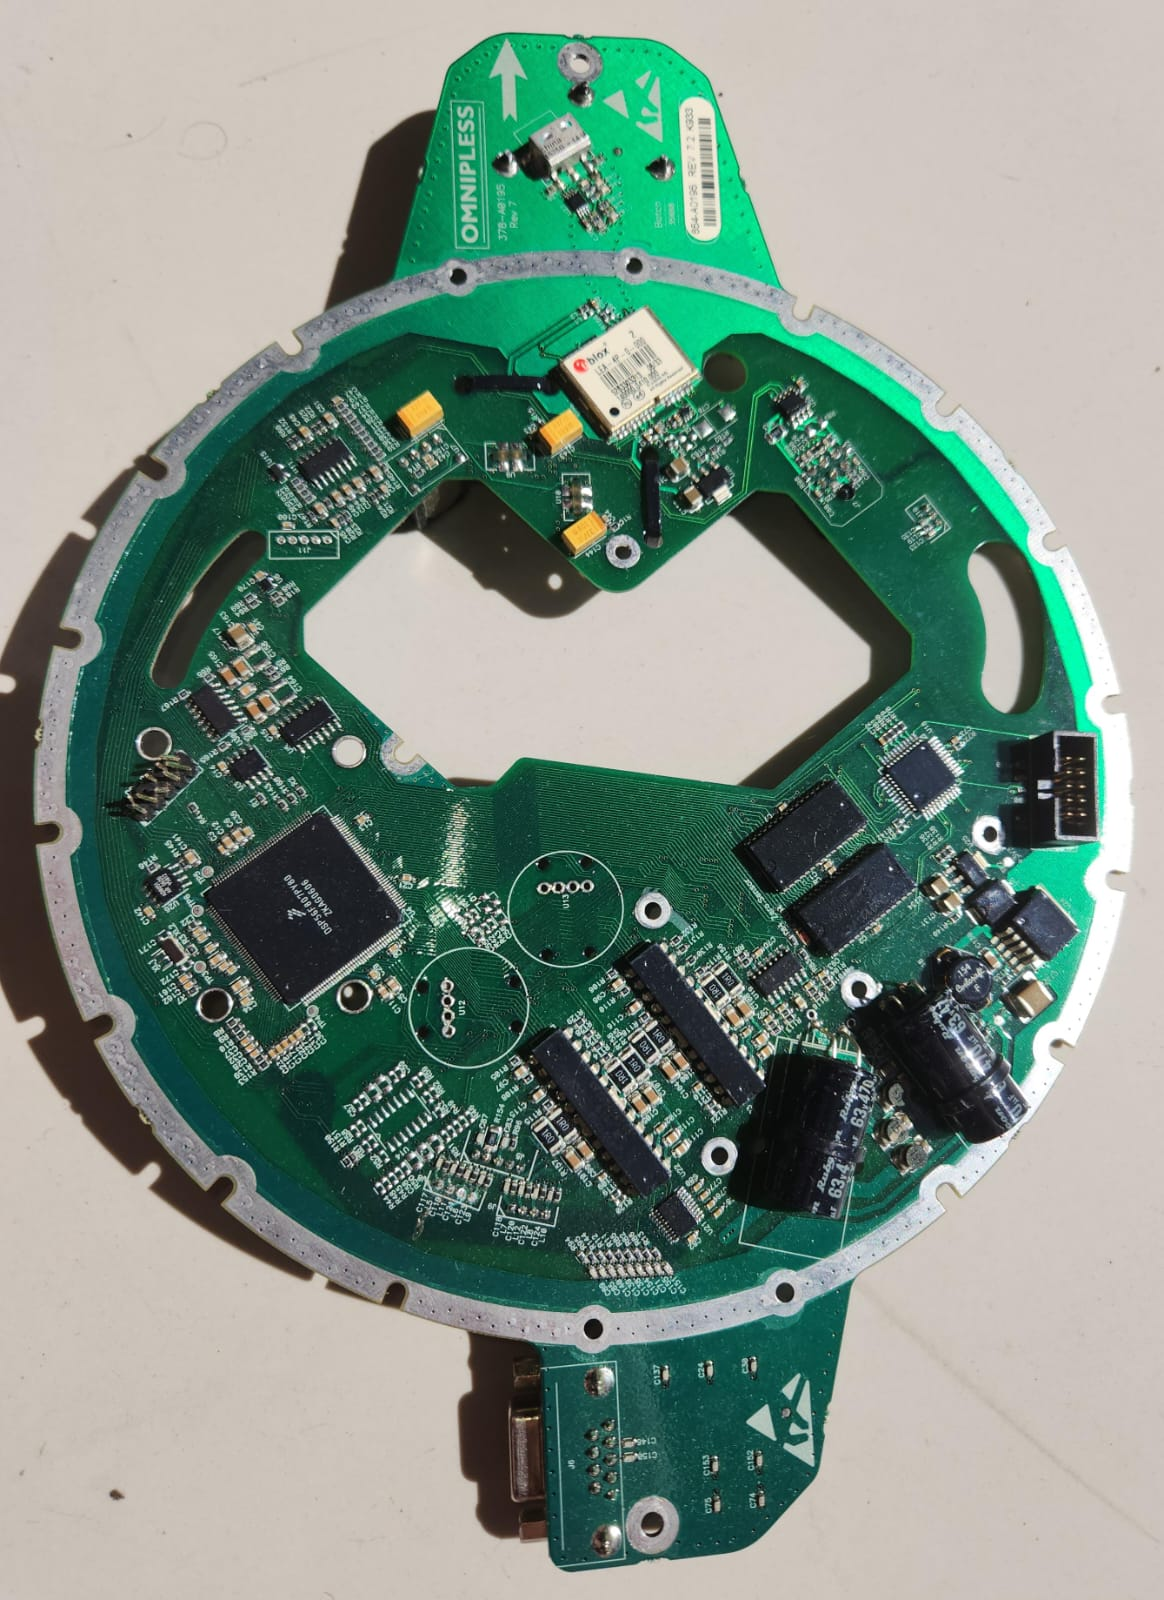
\includegraphics[width=0.4\textwidth, angle=90, origin=c]{gsExistingFront}
  \caption{Existing Antenna Mount PCB (front)}
  \label{fig:gsExistingFront}
\end{figure}
\begin{figure}[!htb]
  \centering
  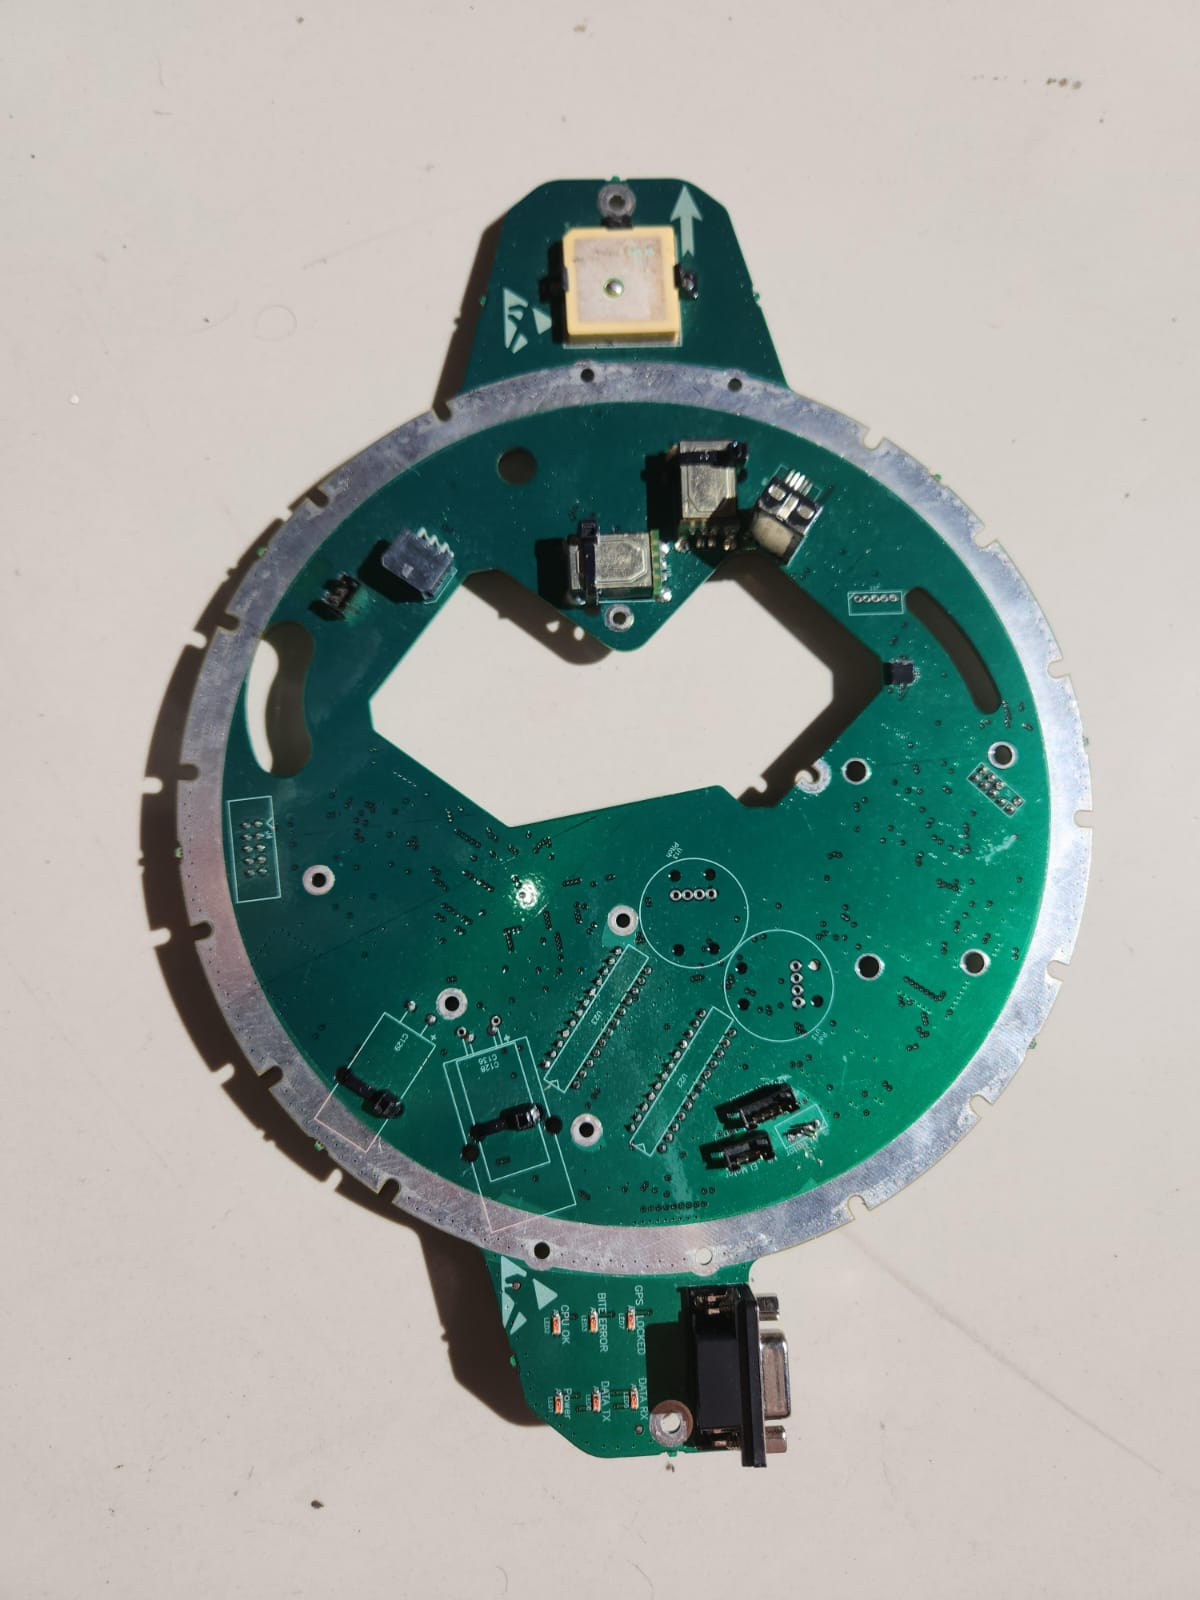
\includegraphics[width=0.4\textwidth, angle=90, origin=c]{gsExistingBack}
  \caption{Existing Antenna Mount PCB (back)}
  \label{fig:gsExistingBack}
\end{figure}
\newpage

\section{PocketQube}\label{sec:appendix_pq}
\begin{figure}[!htb]
    \centering
    \includegraphics[width=0.7\textwidth]{pqBreadboard}
    \caption{PocketQube Breadboard for Testing}
    \label{fig:pqBreadboard}
\end{figure}
\begin{figure}[!htb]
  \centering
  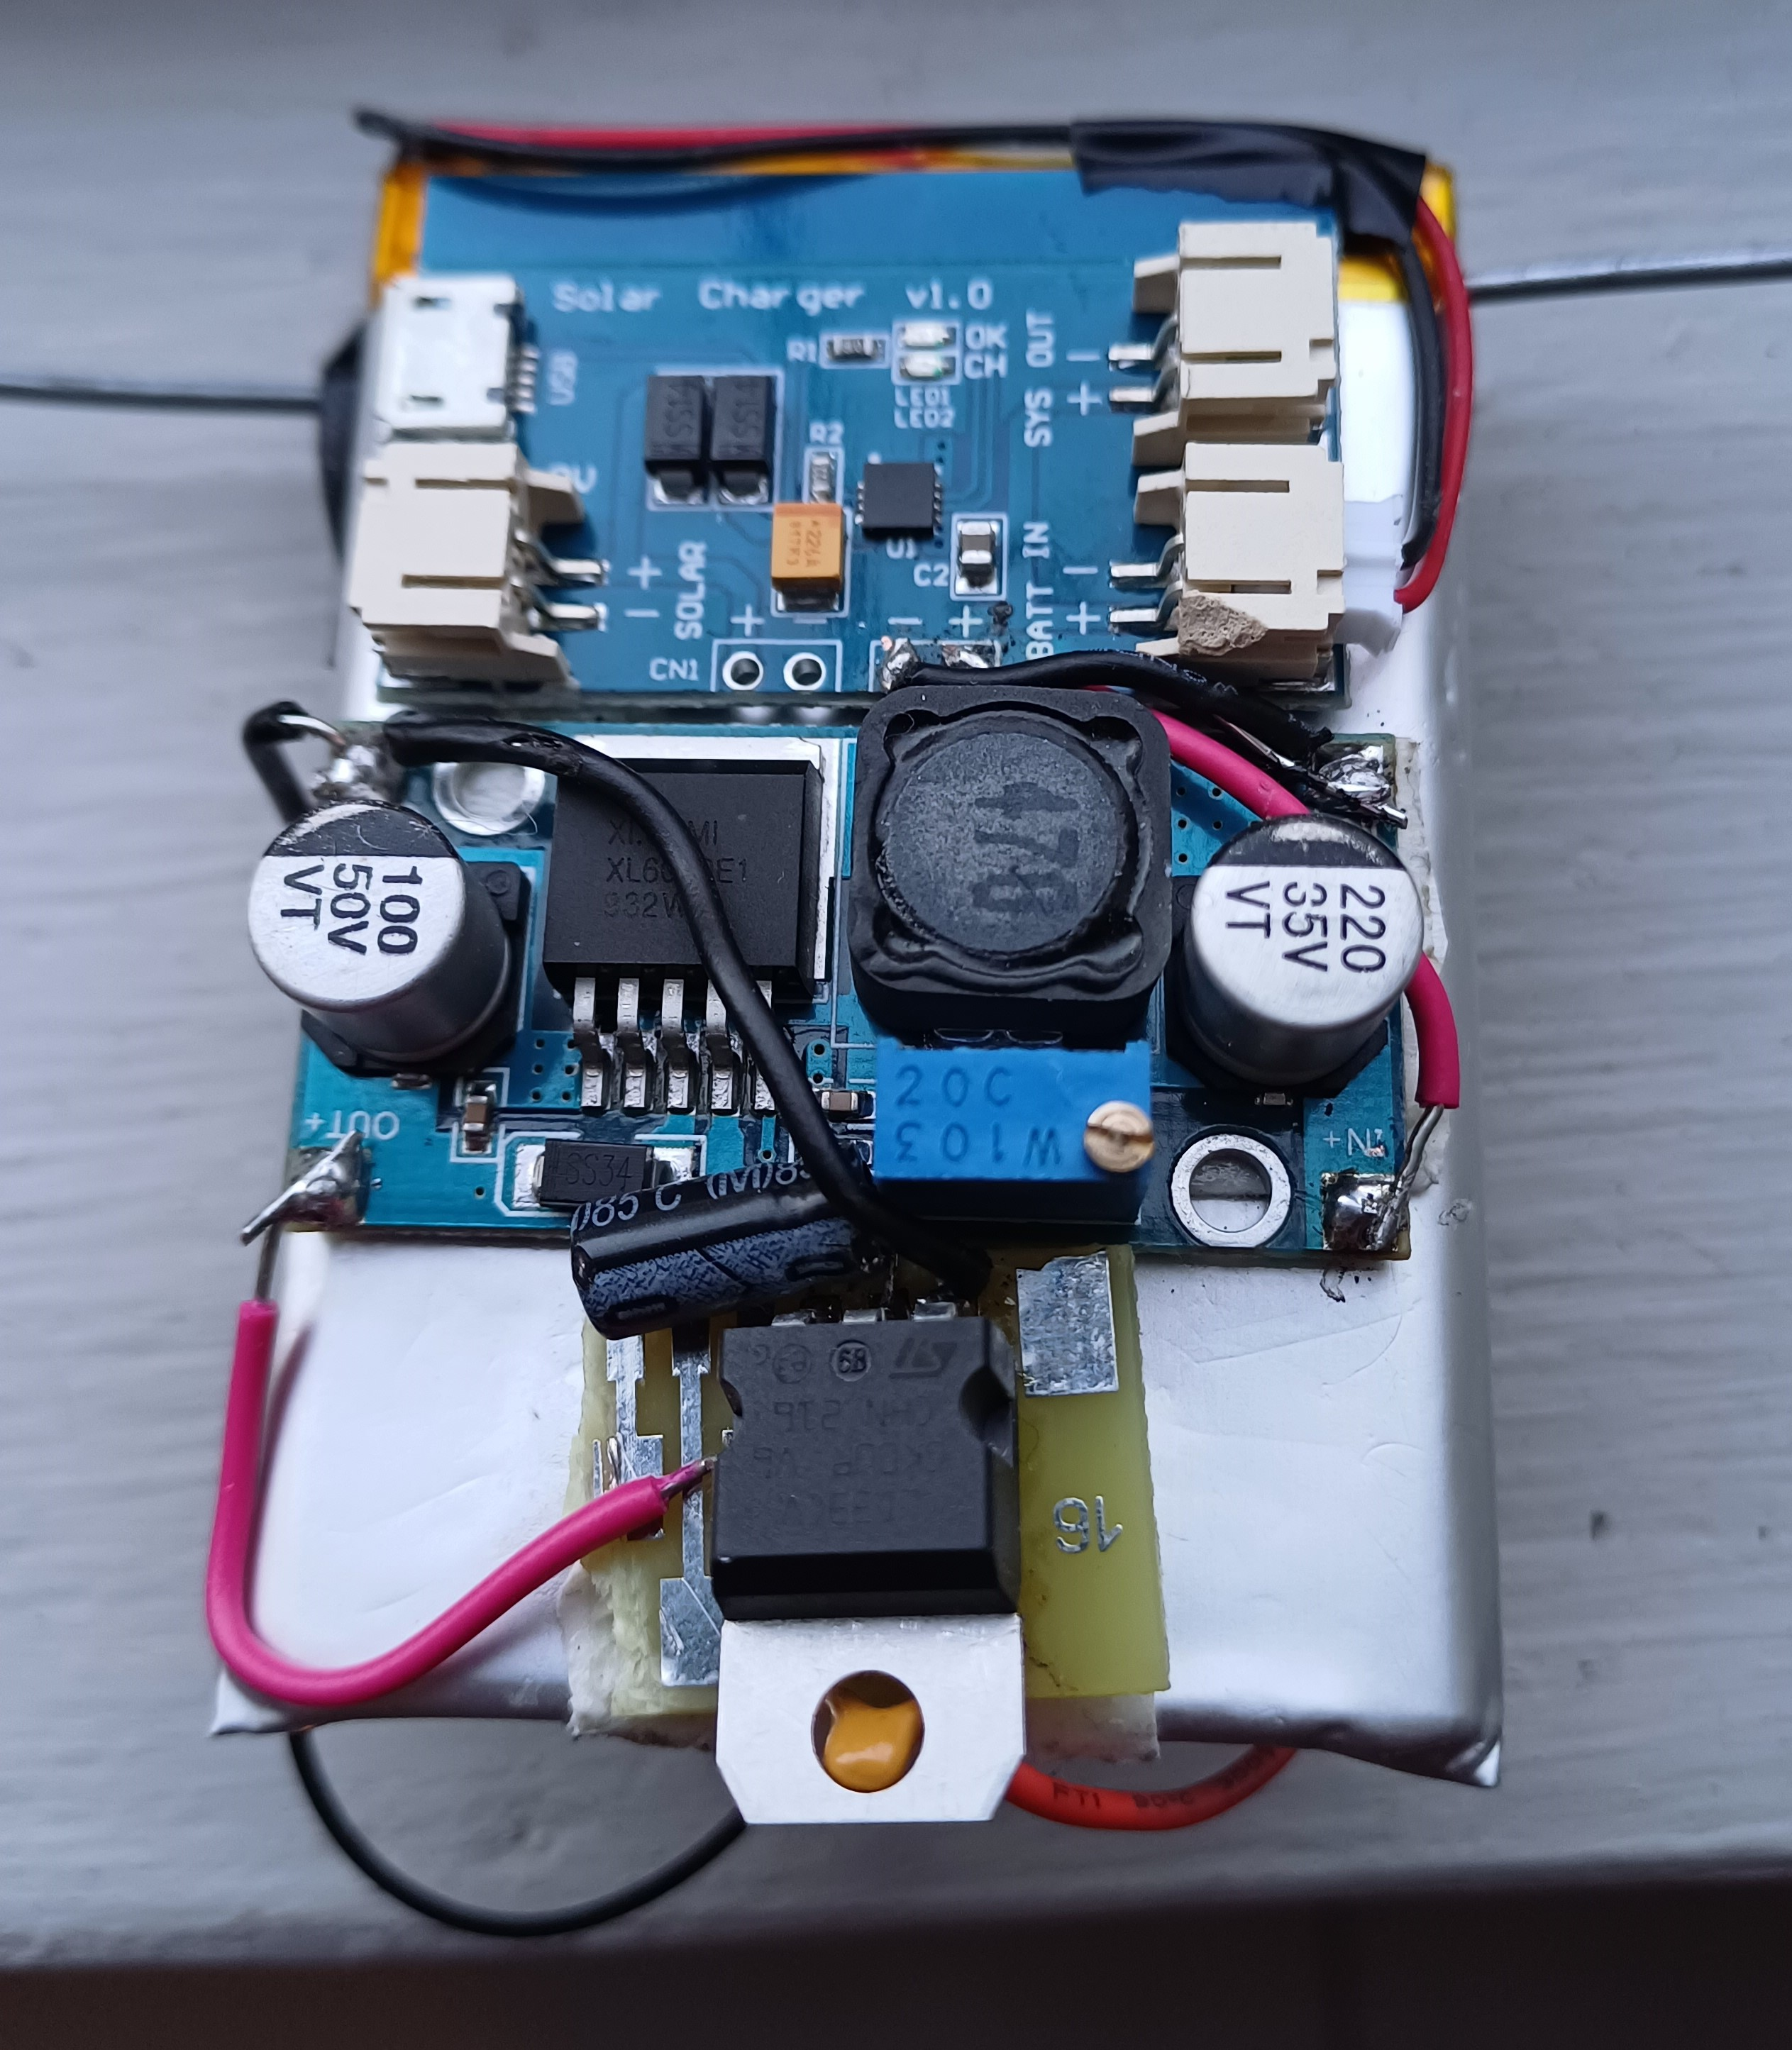
\includegraphics[width=0.4\textwidth,angle=90]{pqUnitPower}
  \caption{PocketQube Unit (back)}
  \label{fig:pqUnitPower}
\end{figure}
\newpage

\section{Mount Specifications}\label{sec:appendix_mount_specifications}
\begin{table}[!htb]
  \centering
  \renewcommand{\arraystretch}{1.2}
  \begin{tabular}{ |c|c| }
  \hline
  \textbf{Component}        & \textbf{Specification}    \\
  \hline
  Motor         & 200 full steps (per 360 degrees) \\ \hline
  Gear A        & 15 teeth \\ \hline
  Gear B        & 20 teeth \\ \hline
  Gear C        & 60 teeth \\ \hline
  Gear D        & 92 inner teeth, 80 outer teeth \\ \hline
  Gear E        & 140 teeth (equivalent) \\ \hline
  \end{tabular}
  \caption{Mount Gear and Motor Specifications}
  \label{tab:mount_specifications}
\end{table}

\section{Mount Rotation}\label{sec:appendix_mount_rotation}
\begin{figure}[!htb]
  \begin{minipage}{.32\textwidth}
    \centering
    \includegraphics[width=0.95\linewidth,angle=270]{mountRotation1}
    \caption{Mount Azimuthal Compensation 1 (Elevation Fixed)}
    \label{fig:mountCompensation1}
  \end{minipage}
  \begin{minipage}{.32\textwidth}
    \centering
    \includegraphics[width=0.95\linewidth,angle=270]{mountRotation2}
    \caption{Mount Azimuthal Compensation 2 (Elevation Fixed)}
    \label{fig:mountCompensation2}
  \end{minipage}
  \begin{minipage}{.32\textwidth}
    \centering
    \includegraphics[width=0.95\linewidth,angle=270]{mountRotation3}
    \caption{Mount Azimuthal Compensation 3 (Elevation Fixed)}
    \label{fig:mountCompensation3}
  \end{minipage}
\end{figure}
\begin{figure}[!htb]
  \begin{minipage}{.32\textwidth}
    \centering
    \includegraphics[width=0.95\linewidth,angle=270]{mountRotation4}
    \caption{Mount Azimuthal Compensation 4 (Elevation Fixed)}
    \label{fig:mountCompensation4}
  \end{minipage}
  \begin{minipage}{.32\textwidth}
    \centering
    \includegraphics[width=0.95\linewidth,angle=270]{mountRotation6}
    \caption{Mount Azimuthal Compensation 5 (Azimuth Fixed)}
    \label{fig:mountCompensation5}
  \end{minipage}
  \begin{minipage}{.32\textwidth}
    \centering
    \includegraphics[width=0.95\linewidth,angle=270]{mountRotation7}
    \caption{Mount Azimuthal Compensation 6 (Azimuth Fixed)}
    \label{fig:mountCompensation6}
  \end{minipage}
\end{figure}
